\documentclass{article}

\usepackage{fullpage}
\usepackage{color}
\usepackage{amsmath}
\usepackage{url}
\usepackage{verbatim}
\usepackage{graphicx}
\usepackage{parskip}
\usepackage{amssymb}
\usepackage{nicefrac}
\usepackage{listings} % For displaying code
\usepackage{algorithm2e} % pseudo-code

\def\rubric#1{\gre{Rubric: \{#1\}}}{}

% Colors
\definecolor{blu}{rgb}{0,0,1}
\def\blu#1{{\color{blu}#1}}
\definecolor{gre}{rgb}{0,.5,0}
\def\gre#1{{\color{gre}#1}}
\definecolor{red}{rgb}{1,0,0}
\def\red#1{{\color{red}#1}}
\def\norm#1{\|#1\|}

% Math
\def\R{\mathbb{R}}
\def\argmax{\mathop{\rm arg\,max}}
\def\argmin{\mathop{\rm arg\,min}}
\newcommand{\mat}[1]{\begin{bmatrix}#1\end{bmatrix}}
\newcommand{\alignStar}[1]{\begin{align*}#1\end{align*}}
\def\half{\frac 1 2}

% LaTeX
\newcommand{\fig}[2]{\includegraphics[width=#1\textwidth]{#2}}
\newcommand{\centerfig}[2]{\begin{center}\includegraphics[width=#1\textwidth]{#2}\end{center}}
\newcommand{\matCode}[1]{\lstinputlisting[language=Matlab]{a2f/#1.m}}
\def\items#1{\begin{itemize}#1\end{itemize}}
\def\enum#1{\begin{enumerate}#1\end{enumerate}}

\begin{document}


\title{CPSC 340 Assignment 4 (due Friday, Nov 2 at 11:55pm)}
\date{}
\maketitle

\vspace{-7em}

\section{Convex Functions}

\enum{
\item $f'(w) = 2\alpha w - \beta$ and $f''(w) = 2\alpha$. Since $2\alpha > 0$, the function is convex.
\item $f'(w) = -\frac{1}{w} $ and $f''(w) = \frac{1}{w^2}$. Since $\frac{1}{w^2} > 0$, the function is convex.
\item $||Xw-y||_1$ and $\frac{\lambda}{2}||w||_1$ are L1 norm so they are convex. Their sum is also convex.
\item $z = -y_iw^Tx_i$ is linear so it is convex. Then $g(z) = \sum_{i=1}^n \log(1+\exp(z))$. Then $g(z) = \frac{e^z}{1+e^z} = 
\frac{1}{1+e^{-z}}$ and $g''(z) = -\frac{1}{(1+e^{-z})^2} \frac{d}{dz}e^{-z} = \frac{e^{-z}}{(1+e^{-z})^2}$ Since
g"(z) is positive, the function is convex.
\item $|w^Tx_i-y_i|$ is a linear function so it is convex. 0 is convex. $\frac{\lambda}{2}||w||^2_2$ is convex because 
$lambda > 0$ and L2 norm is convex. The sum of all of them are also convex.
}

\section{Logistic Regression with Sparse Regularization}

\subsection{L2-Regularization}
L2 Training Error = 0.002, L2 Validation Error = 0.074, Features used: 101, Gradient Iterations: 36

\subsection{L1-Regularization}
L1 Training Error = 0, L2 Validation Error = 0.052, Features used: 71, Gradient Iterations: 78

\subsection{L0-Regularization}
Training error 0.000,
Validation error 0.018,
Features used: 24

\subsection{Discussion}
L0 has the lowest validation error out of all 3 regularizations. This may be because it has the most sparsity out of 
the three and it stops the model from overfitting. However, L0 is considerably slower than the other two because of the
while and for loops.

\subsection{Comparison with scikit-learn}
Scikit-learn's Logistic Regression outputs the same training and validation errors as our own L1 and L2 logistic regression.

\subsection{L$\frac12$ regularization}
\begin{enumerate}
\item $0.5((w-2)^2+0.5)+\lambda\sqrt{|w|}$
\item $w = 2$
\item $w = 0$
\item $w = 1.6$ \\ 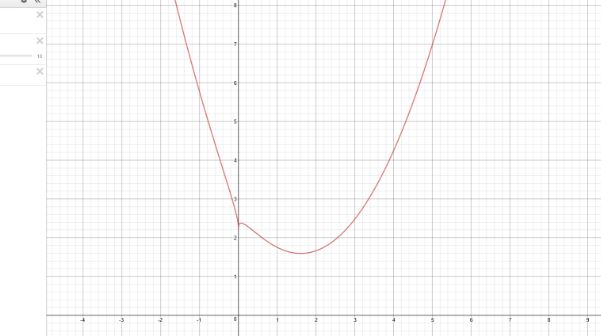
\includegraphics{263.jpg}
\item $w = 0$ \\ 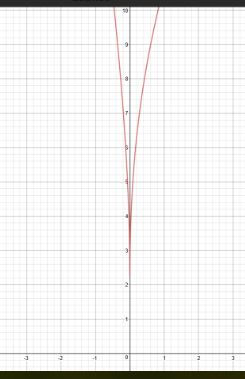
\includegraphics{264.jpg}
\item It behaves more like L1 regularization because there is sparsity in L$\frac12$ regularization
\item It is not a convex optimization as you can see from the graph when $\lambda = 10$, the graph flares outwards.
\end{enumerate}

\section{Multi-Class Logistic}

\subsection{Softmax Classification, toy example}
Class 1: $w_1\dot\hat{x} = 1$\\
Class 2: $w_2\dot\hat{x} = 4$\\
Class 3: $w_3\dot\hat{x} = 2$\\

We would assign 2 to the test example.

\subsection{One-vs-all Logistic Regression}
logLinearClassifier Validation error: 0.070

\subsection{Softmax Classifier Gradient}
\begin{equation*}
    \begin{split}
        f(w) &= \sum_{i=1}^n[-w_{yi}^Tx_i + log(\sum_{c' = 1}^kexp(w_{c'}^Tx_i))]\\
        \frac{\partial}{\partial w_{cj}} &= \sum_{i=1}^n[\frac{\partial}{\partial w_{cj}}(-w_{yi}^Tx_i) + \frac{\partial}{\partial w_{cj}}(log(\sum_{c' = 1}^kexp(w_{c'}^Tx_i)))]\\
        \frac{\partial}{\partial w_{cj}} &= \sum_{i=1}^n[\frac{\partial}{\partial w_{cj}}-(w_{c1}^Tx_{i1}+....+w_{cd}^Tx_{id}) + \frac{\partial}{\partial w_{cj}}(log(\sum_{c' = 1}^kexp(w_{c'}^Tx_i)))]\\
        \frac{\partial}{\partial w_{cj}} &= \sum_{i=1}^n[(-x_{ij}\dot I(y_i = c)) + \frac{\partial}{\partial w_{cj}}(log(\sum_{c' = 1}^kexp(w_{c'}^Tx_i)))]\\
        \frac{\partial}{\partial w_{cj}} &= \sum_{i=1}^n[(-x_{ij}\dot I(y_i = c)) + \frac{exp(w_{c'}^Tx_i)}{\sum_{c' = 1}^kexp(w_{c'}^Tx_i)}\frac{\partial}{\partial w_{cj}}(w_{c'}^Tx_i)]\\
        \frac{\partial}{\partial w_{cj}} &= \sum_{i=1}^n[(-x_{ij}\dot I(y_i = c)) + \frac{exp(w_{c'}^Tx_i)}{\sum_{c' = 1}^kexp(w_{c'}^Tx_i)}x_{ij}]\\
        \frac{\partial}{\partial w_{cj}} &= \sum_{i=1}^n[(x_{ij}(p(y_i = c | W, x_i) - I(y_i = c))]\\
    \end{split}
\end{equation*}

\subsection{Softmax Classifier Implementation}
Validation error: 0.008

\subsection{Comparison with scikit-learn, again}
One vs All: Training error 0.084, Validation error 0.070
Softmax Function: Training error 0.000, Validation error 0.016

Scikit Learn's Implementation of One vs All yields the exact same validation error as our own logLinearClassifier. However,
their validation error for sotmax classifier is actually double our validation error.

\subsection{Cost of Multinomial Logistic Regression}
\begin{enumerate}
    \item Every iteration of gradient descent runs over O(n) examples. Each example costs O(dk) because we need to 
    compute $w^Tx_i$, which is O(d) for k values. The iterations of gradient descent is given by O(T) so we have
    O(Tndk).
    \item We need O(dk) to classify one example. Since there are t test examples its, O(tdk) 
\end{enumerate}

\section{Very-Short Answer Questions}

\enum{
\item This is difficult to do because "relevance" is hard to define. Features may only be "relevant" in the context of
other features. It also becomes more difficult if there is collinearity between features because we wouldn't know which
feature to pick. Other issues that make it difficult may be conditional independence; where features can be irrelevant 
given other features.
\item This is similar to the first answer where a feature may be colinear with another feature so both would be selected.
Another problem with this is that feature 1 may depend on feature 2 and only feature 1 is picked. Then it wouldm't make 
sense if feature 1 was picked without feature 2.
\item We would use L1-loss in datasets with a lot of outlier points and we would use L1-regularization in datasets that 
contain irrelevant features 
\item L1 and L2 regularization are convex. Only L2 regularization yield unique solutions. L1 and L0 regularizations yield
sparse solutions. 
\item Increasing $\lambda$ directly increases sparsity. Small lambda selects more features which causes Training Error to 
go down while approxiamation error goes down. Large lambda selects fewer features which can be a better approximation of the test data so approxiamation error
decreases and training error increases. 
\item We can try using the bootstrap method. We would run the feature selection on each sample. Each run would give us a set 
of features and we would use the union of all the sets of features. This allows us to take all the features in the bootstrap, so it allows us
to grab all relevant features
\item This means that all the classes can be separated by a hyperplane
\item If we want to minimize the number of classification error, we would use the 0-1 Loss. However, the 0-1 Loss is non-smooth
and not convex. We use logistic loss for its convexity and smoothness so we can minimize this with gradient descent.
\item Support vectors are vectors from the closest points to the boundary. These are useful because we can use them to find the boundary
with the maximum distance from each point. 
\item Perceptron will only work for linear models that have linearly separable datasets
\item Multiclass classifiers are better when there may be more than one "correct" class label and we can fit "k" binary classifers.
\item The $\sigma$ controls the width of the bumps. The smaller the $\sigma$, the more complicated the model is. As the model gets 
more complicated, it will start to overfit and training error goes up. On the other side, for larger $\sigma$, we will have higher
training error but lower approxiamation error.
}

\end{document}